\documentclass[11pt]{article}

% -------------------------------------------------------------- packages
\usepackage[margin=1in]{geometry}
\usepackage{amsmath, amssymb}
\usepackage{graphicx}
\usepackage{booktabs}
\usepackage{array}
\usepackage{caption}
\usepackage{subcaption}
\usepackage{float}
\usepackage{hyperref}
\usepackage{xcolor}
\hypersetup{colorlinks=true, linkcolor=blue!50!black,
            citecolor=blue!50!black, urlcolor=blue!50!black}
\usepackage{enumitem}
\setlist{itemsep=2pt, topsep=2pt}

\graphicspath{{figures/}}

% -------------------------------------------------------------- title
\title{Capital Bikeshare Hourly Demand:\\
       Exploratory Data Analysis Report}
\author{STAT 24620 / FINM 34700 / STAT 32950 --- Group Project (Draft)}
\date{Spring 2026}

\begin{document}
\maketitle

% =====================================================================
\section{Introduction and research question}

We work with the \emph{Capital Bikeshare hourly demand} dataset
(\texttt{bike\_sharing\_hourly.csv}, UCI Machine Learning Repository).
It records every hour of operation of the Washington D.C.\ bikeshare
system between 2011-01-01 and 2012-12-31, together with calendar and
weather covariates. The target is \texttt{cnt}, the total number of
rentals during the hour.

\paragraph{Tentative research question.}
\emph{What drives hourly bike-rental demand in Washington D.C., and how
do calendar and weather variables jointly shape it?} Concretely:
(i) discover the dominant patterns in hourly demand using a
multivariate-structure method (PCA / clustering) and (ii) quantify and
predict demand using a supervised method (regression / random forest),
then compare the two views.

\paragraph{Data at a glance.}
The CSV has $n = 17{,}379$ rows and 18 columns with \emph{no missing
values}. Columns: calendar (\texttt{dteday}, \texttt{season},
\texttt{yr}, \texttt{mnth}, \texttt{hr}, \texttt{holiday},
\texttt{weekday}, \texttt{workingday}), weather (\texttt{weathersit},
\texttt{temp}, \texttt{atemp}, \texttt{hum}, \texttt{windspeed}), and
counts (\texttt{casual}, \texttt{registered}, \texttt{cnt}). By
definition $\texttt{cnt}=\texttt{casual}+\texttt{registered}$, so the
two components may not be used as predictors of \texttt{cnt}. A derived
binary label \texttt{high\_demand} flags hours above the sample median.

Two minor facts inform downstream choices. First, the file actually
contains $17{,}379 < 17{,}544 = 731 \times 24$ rows: \textbf{165
day-hours are absent from the table}, which we treat as zero-rental
hours (consistent with the \texttt{cnt} minimum of $1$). Second, the
weather variables are pre-normalized to $[0,1]$ by the UCI provider; we
de-normalize them only for plotting.

This report has two parts. \textbf{Part 1} (\S\S2--6) is the classical
descriptive EDA: distributions, time series, hour-of-day patterns,
weather and calendar effects, correlation, and the binary label.
\textbf{Part 2} (\S\S7--12) is a deeper multivariate-structure
exploration: mutual information, temporal dependence, variance
decomposition, PCA / K-means / hierarchical / t-SNE on day-level
24-hour profiles, hour~$\times$~temperature interaction surface, and
Mahalanobis multivariate outliers.

% =====================================================================
\part*{Part 1 --- Classical descriptive EDA}
\addcontentsline{toc}{section}{Part 1 -- Classical descriptive EDA}

% =====================================================================
\section{Target variable, time series, and basic patterns}

\paragraph{Marginal distribution.}
Hourly \texttt{cnt} ranges from $1$ to $977$ with mean $189.5$ and sd
$181.4$ (median $142$). The raw distribution is strongly right-skewed
(skewness $= 1.28$, excess kurtosis $= 1.42$;
Figure~\ref{fig:cnt-dist}, left). After $\log(1+\texttt{cnt})$ the
skewness drops to $-0.82$, but the distribution becomes clearly
\emph{bimodal} (right) --- a hint of two latent demand regimes that
Part 2 will recover quantitatively.

\begin{figure}[H]
\centering

\includegraphics[width=0.92\linewidth]{fig01_cnt_distribution.pdf}
\caption{Raw vs.\ log-transformed hourly demand.}
\label{fig:cnt-dist}
\end{figure}

\paragraph{Long-term trend and seasonality.}
Two years of data (2011--2012) show three time-scales of variation
(Figures~\ref{fig:daily}--\ref{fig:monthly}): a positive
\emph{year-over-year trend} (mean hourly demand jumps from $\sim 144$
in 2011 to $\sim 235$ in 2012, $+63\%$), an \emph{annual cycle}
peaking in summer/fall and dipping in winter, and \emph{sharp
single-day dips} on bad-weather days (Hurricane Sandy in late October
2012 is visible).

\begin{figure}[H]
\centering
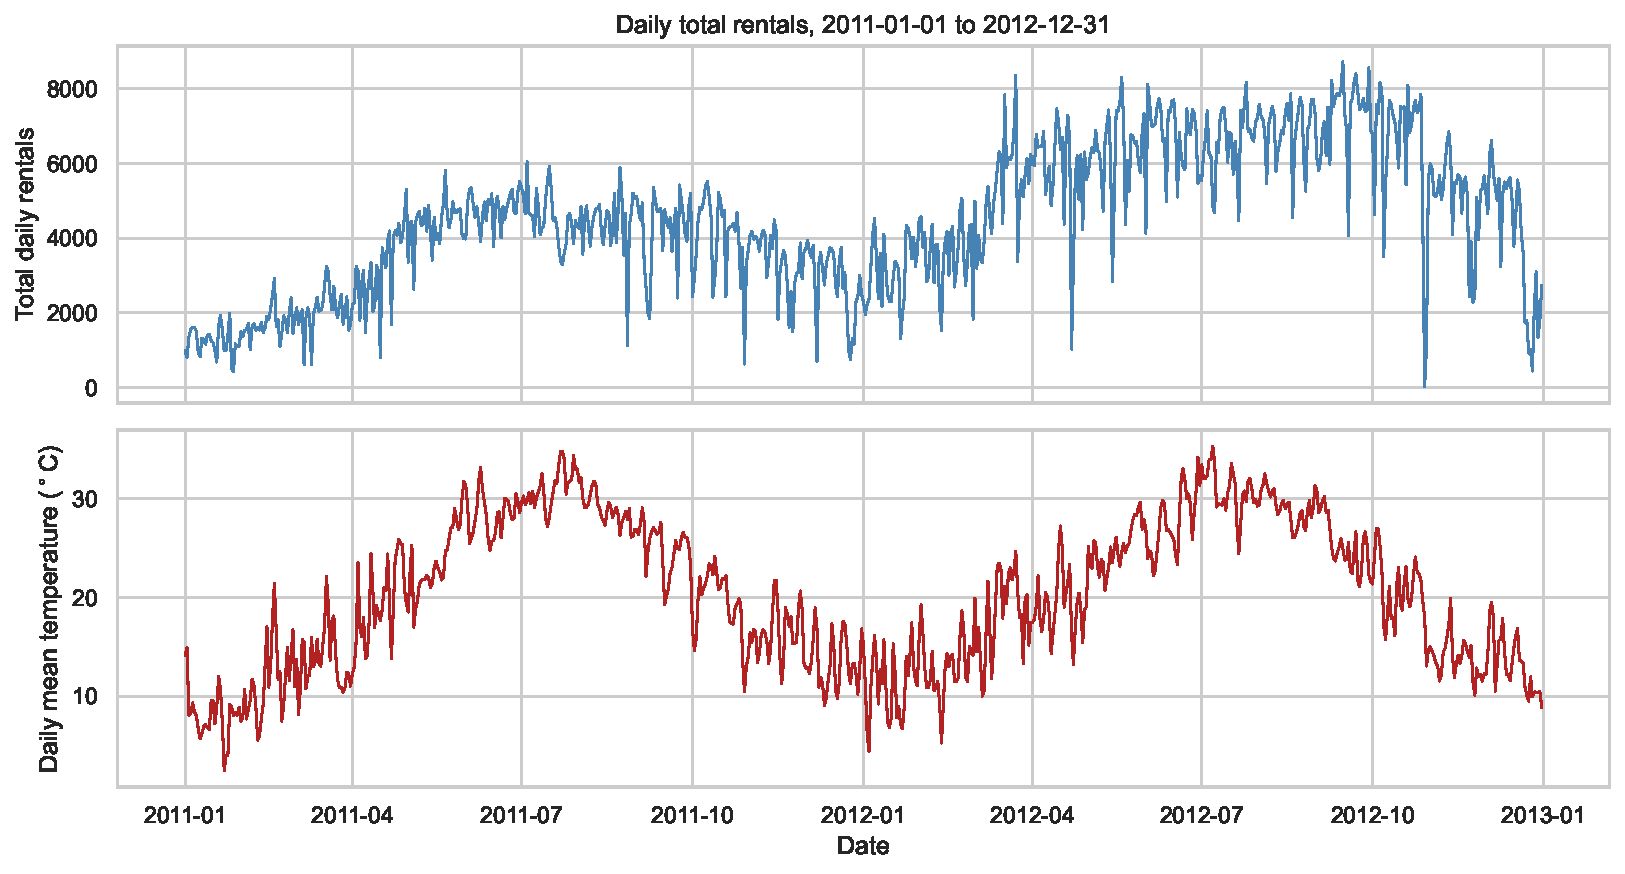
\includegraphics[width=0.92\linewidth]{fig02_daily_timeseries.pdf}
\caption{Daily total rentals (top) and daily mean temperature (bottom).}
\label{fig:daily}
\end{figure}

\begin{figure}[H]
\centering
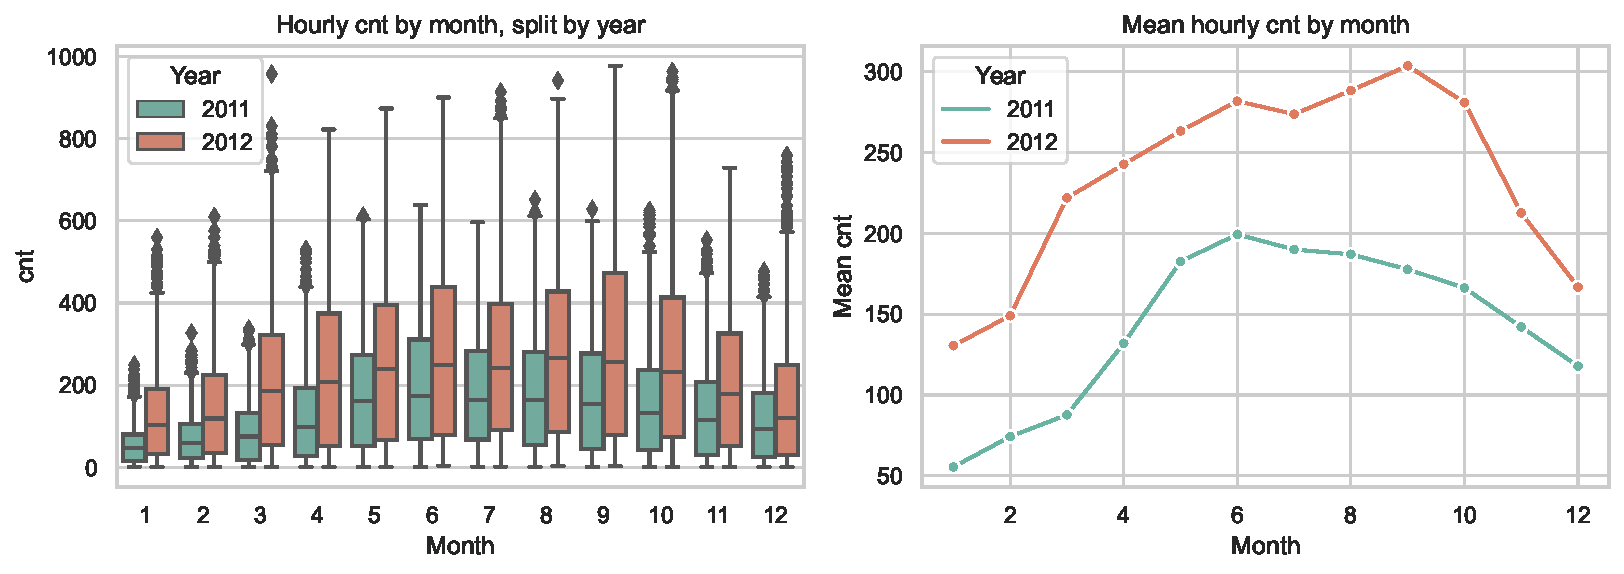
\includegraphics[width=0.92\linewidth]{fig03_monthly_pattern.pdf}
\caption{Hourly \texttt{cnt} by month, split by year.}
\label{fig:monthly}
\end{figure}

% =====================================================================
\section{Hour-of-day structure}

The data's most distinctive feature is its intraday shape
(Figures~\ref{fig:hourly}--\ref{fig:heatmap}). On working days demand
follows a sharp \emph{bimodal commuter signature}: peaks at 08:00 and
17:00--18:00. On weekends/holidays the curve collapses to a single
broad daytime hump centered around 12:00--15:00. Season mostly
\emph{scales} the curve, while \texttt{workingday} \emph{reshapes} it,
strongly suggesting an \texttt{hr}~$\times$~\texttt{workingday}
interaction.

\begin{figure}[H]
\centering
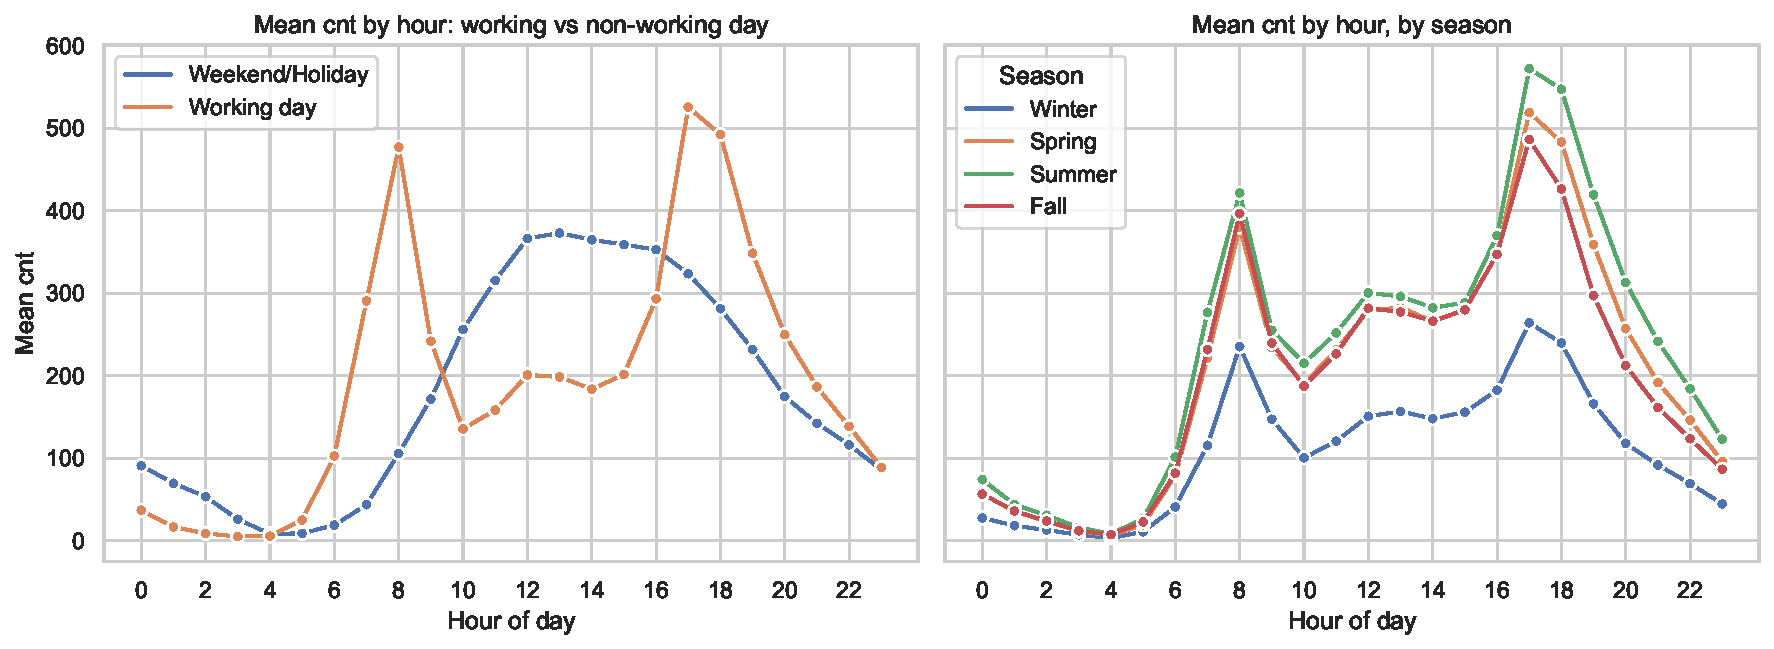
\includegraphics[width=0.92\linewidth]{fig04_hourly_by_workingday_season.pdf}
\caption{Mean \texttt{cnt} by hour. Left: by working-day status.
Right: by season.}
\label{fig:hourly}
\end{figure}

\begin{figure}[H]
\centering
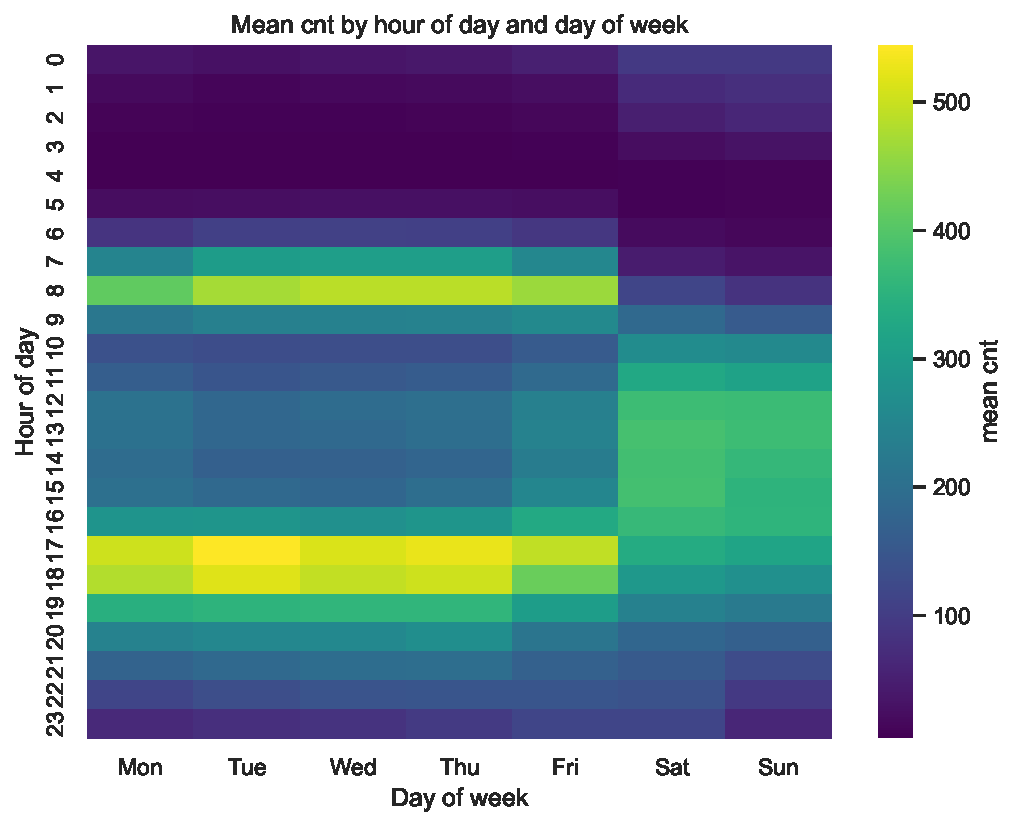
\includegraphics[width=0.55\linewidth]{fig05_hour_weekday_heatmap.pdf}
\caption{Hour~$\times$~weekday heatmap of mean \texttt{cnt}.}
\label{fig:heatmap}
\end{figure}

% =====================================================================
\section{Weather effects}

\begin{figure}[H]
\centering
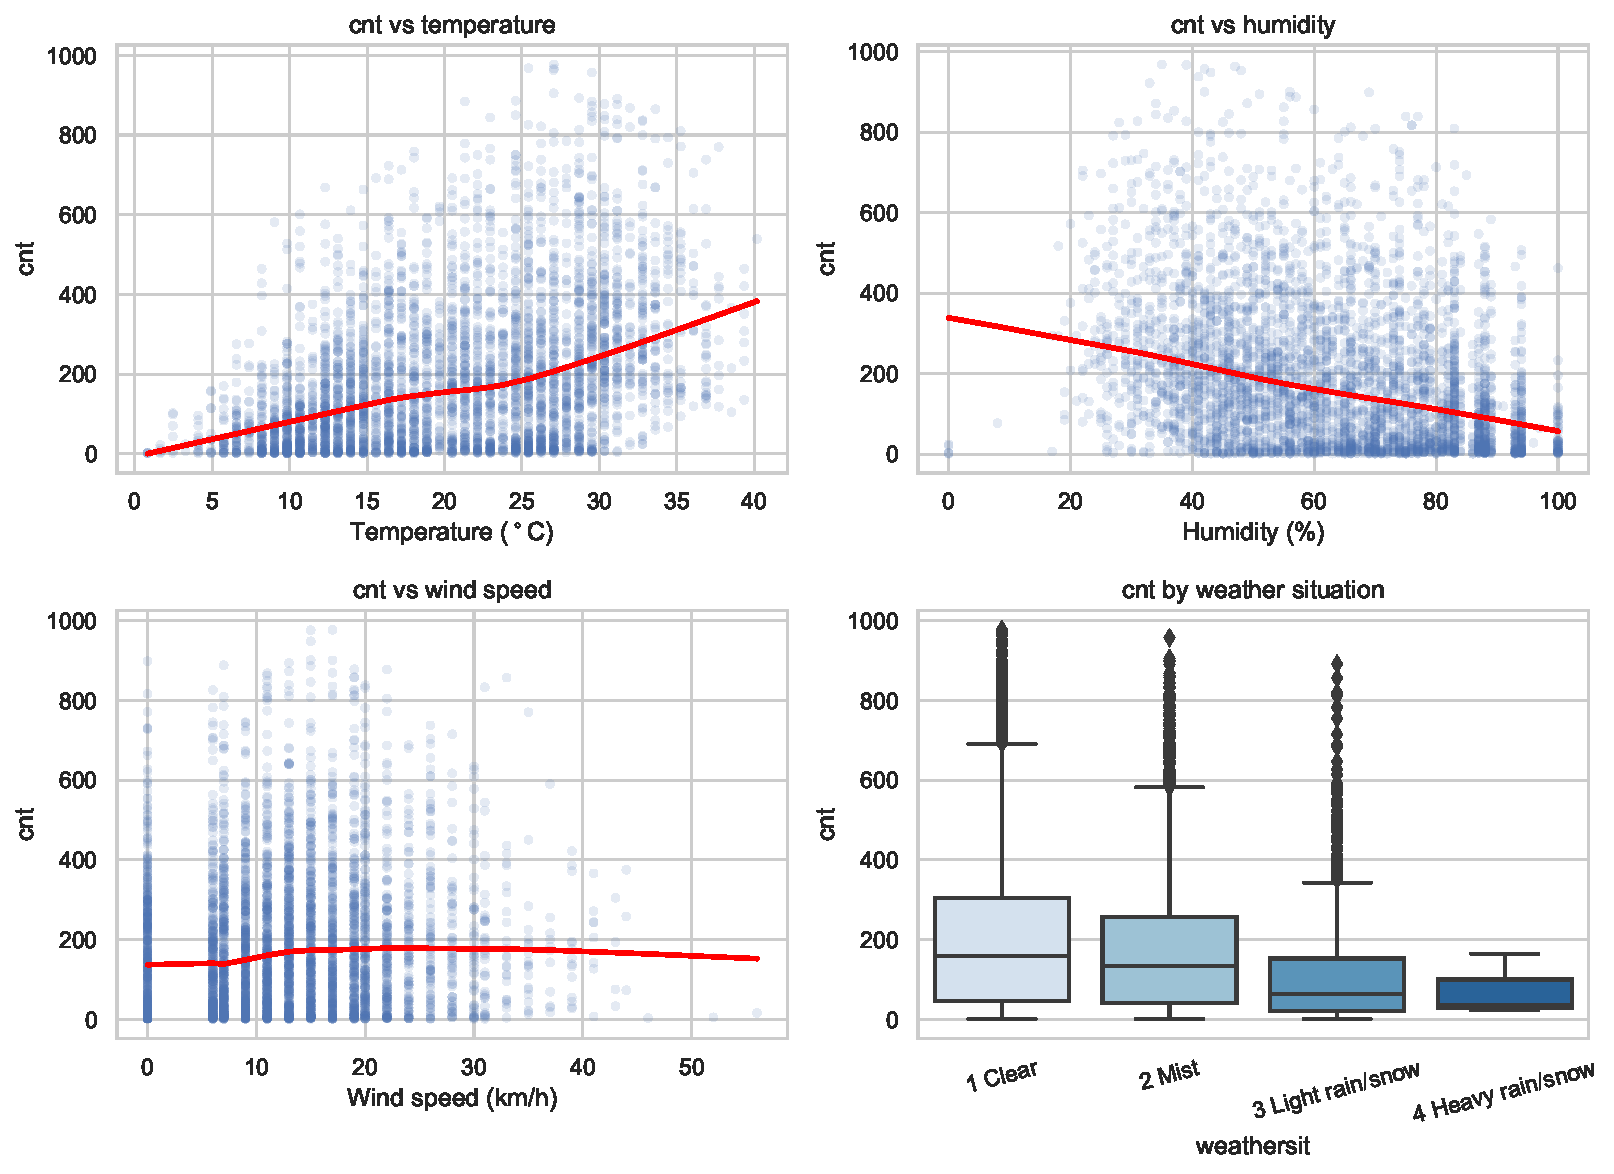
\includegraphics[width=0.92\linewidth]{fig06_weather_effects.pdf}
\caption{Weather effects on hourly demand. Red curves are LOWESS
smooths.}
\label{fig:weather}
\end{figure}

\begin{itemize}
\item Temperature is strongly positive, roughly linear up to
      $\sim 30^\circ$C and slightly concave above.
\item Humidity is clearly negative, especially above 80\%.
\item Wind speed is weakly negative.
\item \texttt{weathersit} decreases monotonically from category 1
      (clear) to 3 (light rain/snow). Category 4 has \emph{3 hours
      total} in the two-year sample and must be merged with category 3
      for modeling.
\end{itemize}

% =====================================================================
\section{Calendar effects and casual vs.\ registered}

\begin{figure}[H]
\centering
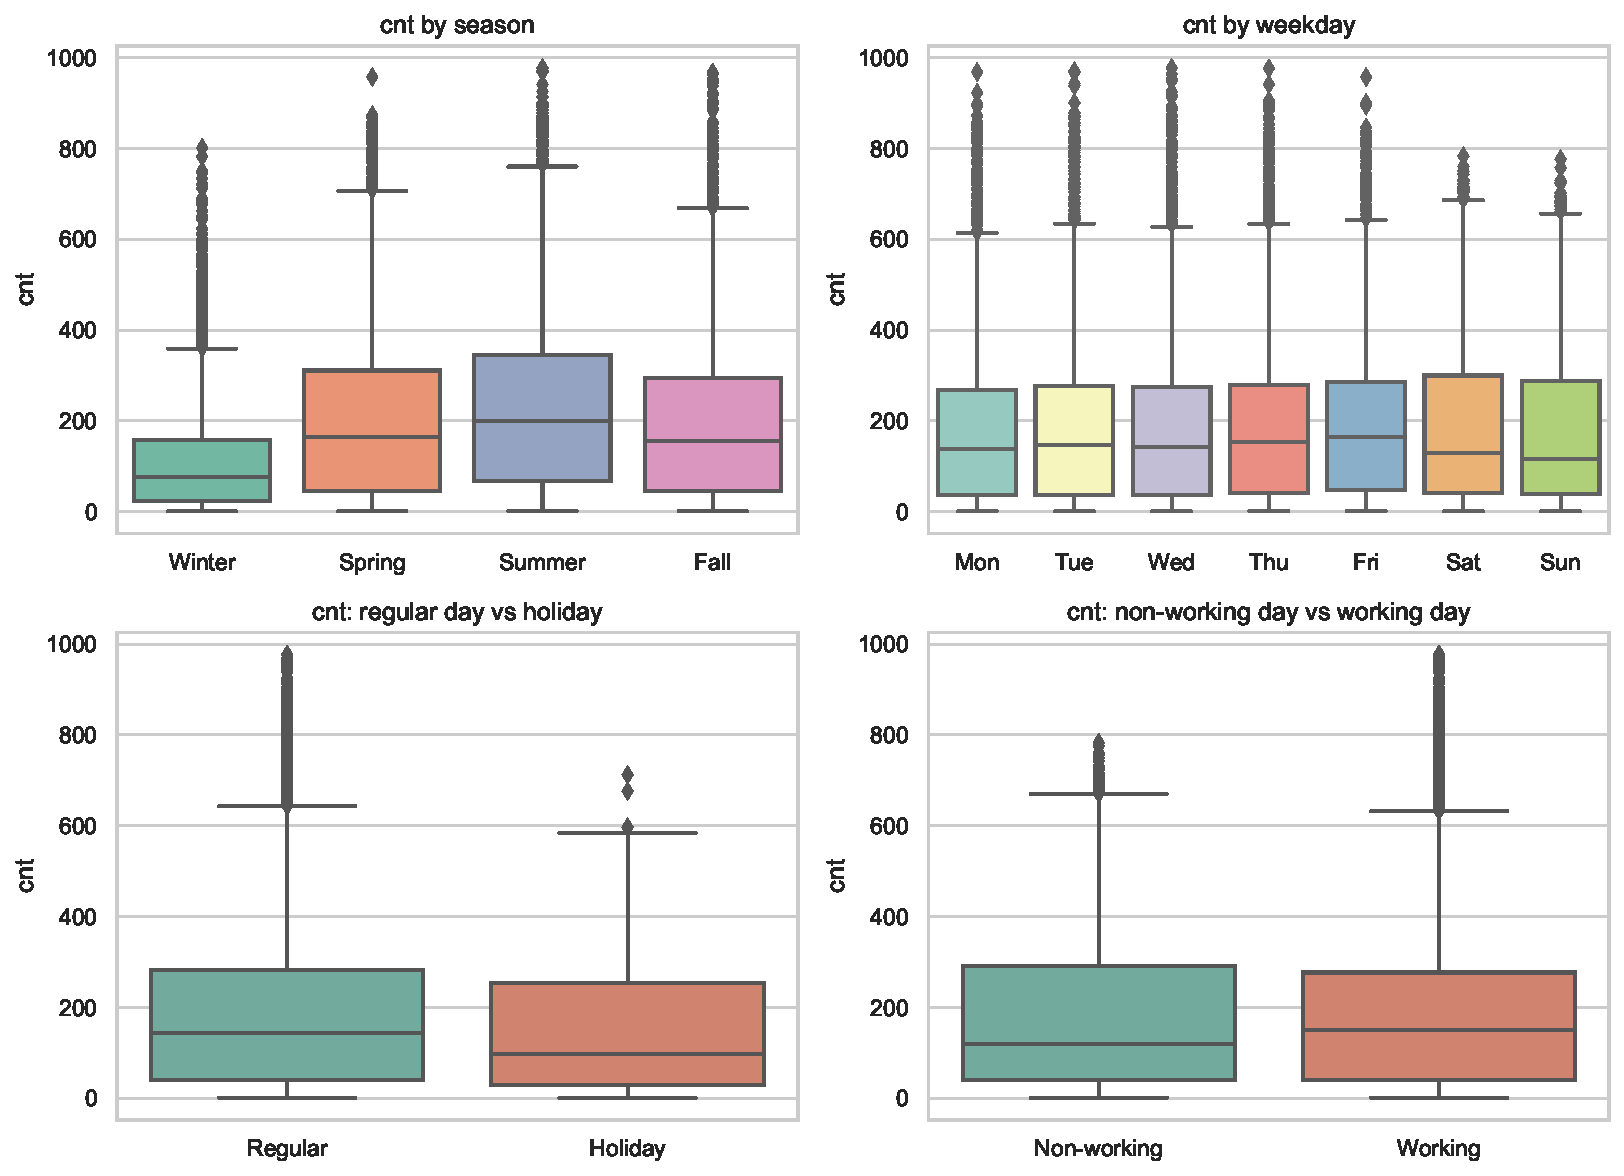
\includegraphics[width=0.85\linewidth]{fig07_categorical_effects.pdf}
\caption{Marginal effect of season, weekday, holiday, workingday.}
\label{fig:cat}
\end{figure}

Weekday-level marginal boxplots are surprisingly flat --- the
\emph{shape}, not the daily total, is what differentiates weekdays
from weekends. Splitting demand into the two user types
(Figure~\ref{fig:casreg}) explains why: registered users drive the
bimodal commuter signature, while casual users surge on weekends.
\texttt{cnt} is effectively a mixture of these two latent populations.

\begin{figure}[H]
\centering
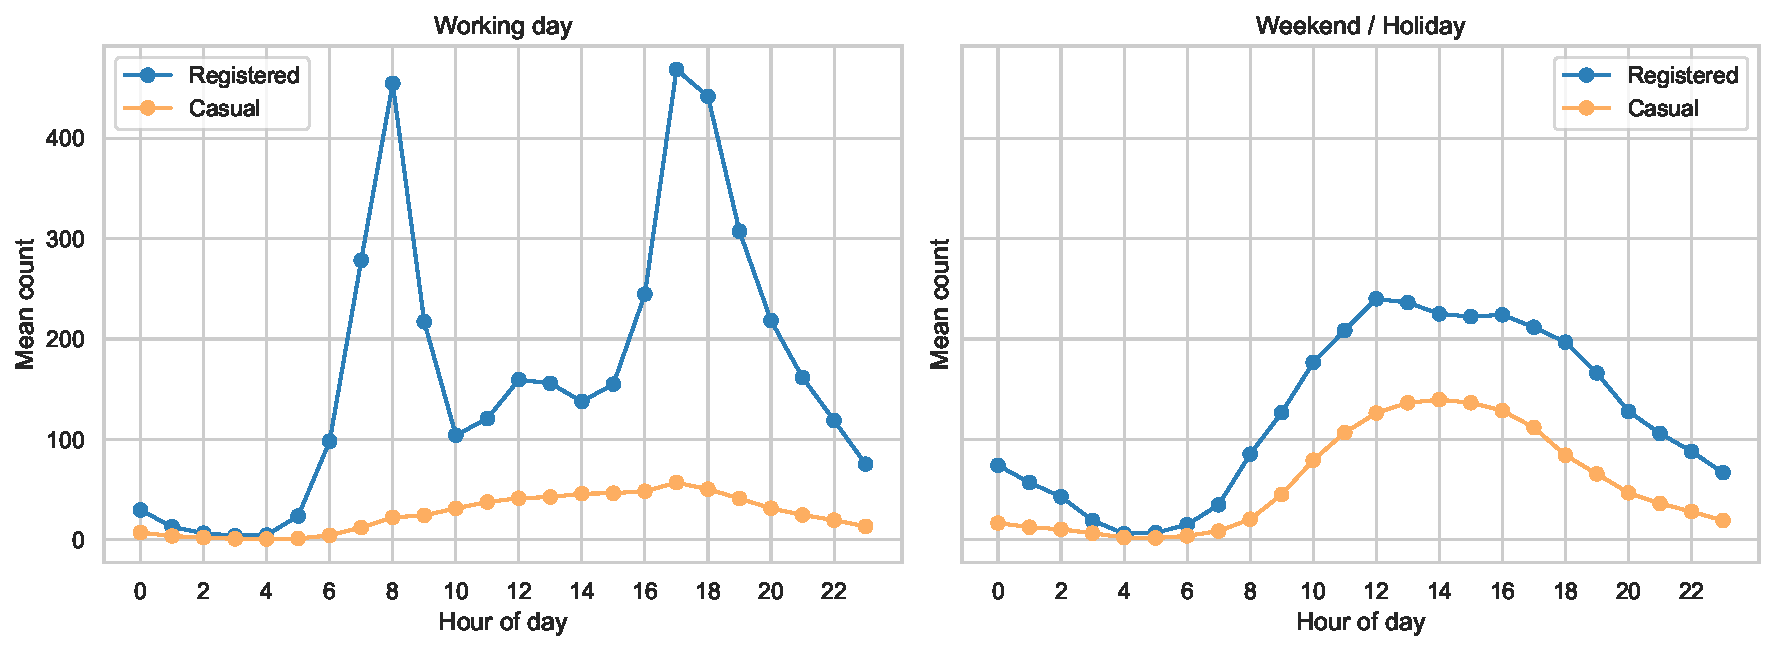
\includegraphics[width=0.92\linewidth]{fig08_casual_vs_registered.pdf}
\caption{Mean hourly casual vs.\ registered demand, split by working
day status.}
\label{fig:casreg}
\end{figure}

% =====================================================================
\section{Correlation, redundancy, and the binary label}

Two redundancies dominate the correlation matrix
(Figure~\ref{fig:corr}): \texttt{temp}~$\approx$~\texttt{atemp}
($r = 0.988$, Figure~\ref{fig:tempatemp}) and
\texttt{season}~$\approx$~\texttt{mnth} ($r = 0.83$). \texttt{cnt}
correlates most strongly with \texttt{temp}/\texttt{atemp} ($\sim 0.40$),
\texttt{hr} ($0.39$), and \texttt{yr} ($0.25$); the linear correlation
with \texttt{hr} is \emph{misleadingly small} because the relationship
is bimodal --- a fact Part~2 will quantify with mutual information.

\begin{figure}[H]
\centering
\begin{subfigure}{0.60\linewidth}
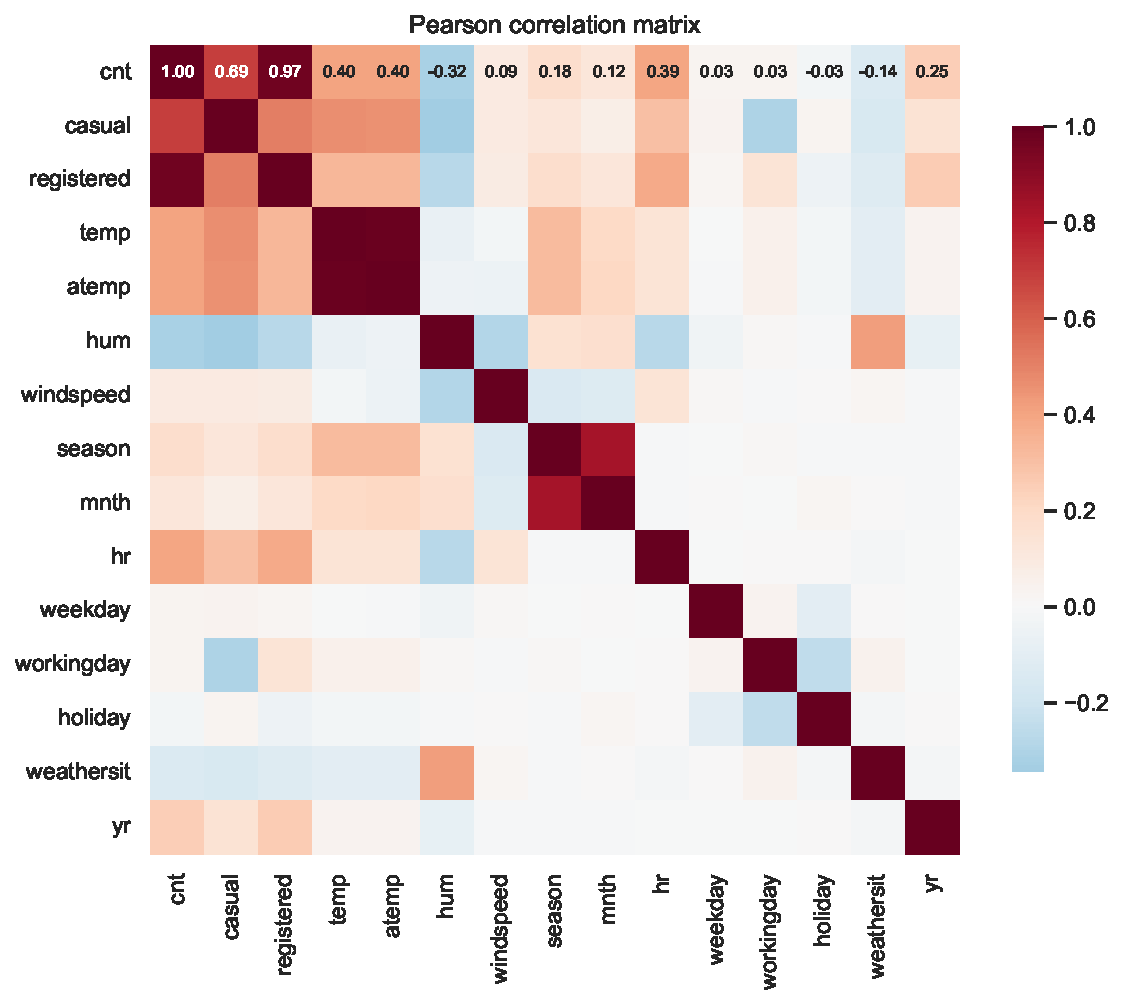
\includegraphics[width=\linewidth]{fig09_correlation_matrix.pdf}
\caption{Pearson correlation matrix.}\label{fig:corr}
\end{subfigure}
\hfill
\begin{subfigure}{0.36\linewidth}
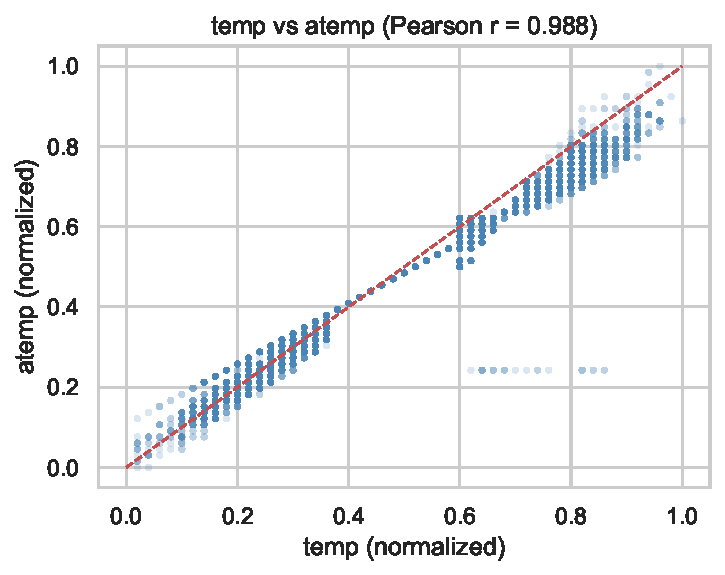
\includegraphics[width=\linewidth]{fig10_temp_atemp.pdf}
\caption{\texttt{temp} vs.\ \texttt{atemp}.}\label{fig:tempatemp}
\end{subfigure}
\caption{Linear-correlation diagnostics.}
\end{figure}

\paragraph{Heteroskedasticity and the binary label.}
Boxplots of \texttt{cnt} by hour (Figure~\ref{fig:hourbox}) show
spread that grows with the mean, indicating heteroskedasticity: any
linear model should be fit on $\log(1+\texttt{cnt})$, or replaced by
a method that does not assume constant variance. The derived
\texttt{high\_demand} label is essentially balanced (49.9\%
\texttt{High}, 50.1\% \texttt{Low}), so no re-sampling tricks are
needed for a classification benchmark.

\begin{figure}[H]
\centering
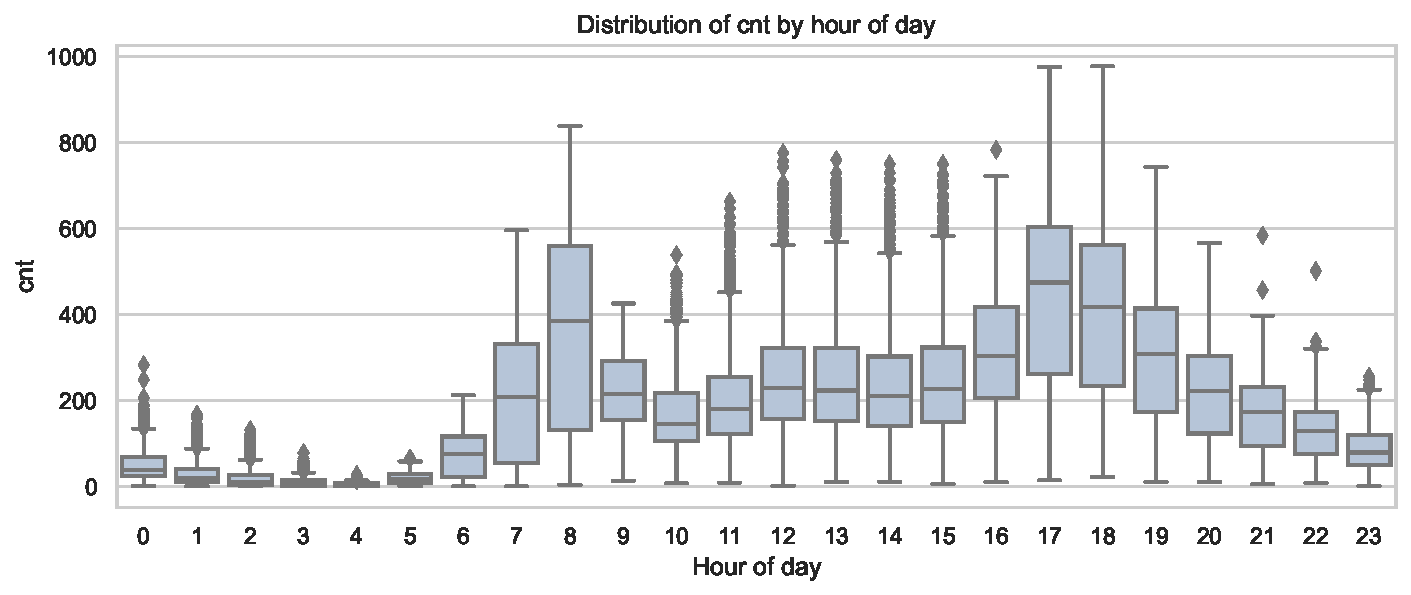
\includegraphics[width=0.82\linewidth]{fig11_cnt_by_hour_box.pdf}
\caption{Heteroskedasticity: variance of \texttt{cnt} grows with
hour-of-day mean.}\label{fig:hourbox}
\end{figure}

% =====================================================================
\part*{Part 2 --- Multivariate structure exploration}
\addcontentsline{toc}{section}{Part 2 -- Multivariate structure}

Part 1 stopped at pairwise relationships. Part 2 looks for
\emph{joint} structure that no single bivariate plot can reveal.

% =====================================================================
\section{Non-linear dependence: mutual information vs.\ Pearson}

Pearson correlation captures only linear dependence; the bimodal
\texttt{hr}~$\to$~\texttt{cnt} curve has zero linear slope on average.
Mutual information $I(X;Y)$ captures \emph{any} statistical dependence
and so should re-rank \texttt{hr} much higher
(Figure~\ref{fig:mi}).

\begin{figure}[H]
\centering
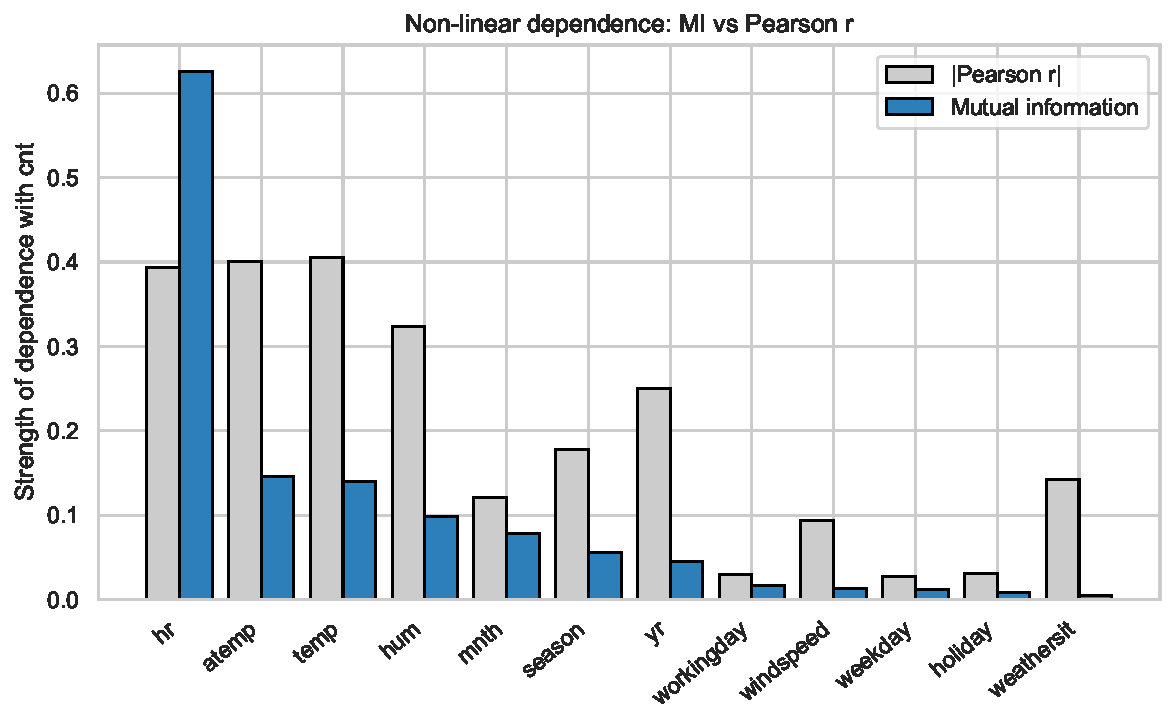
\includegraphics[width=0.85\linewidth]{fig12_mutual_info.pdf}
\caption{Mutual information (blue) vs.\ absolute Pearson correlation
(grey) between each predictor and \texttt{cnt}.}\label{fig:mi}
\end{figure}

\paragraph{Findings.} \texttt{hr} jumps to the top of the MI ranking
despite a modest $|r|\approx 0.39$. \texttt{workingday} and
\texttt{weekday}, which shift the \emph{shape} of the hourly curve
without shifting its overall mean, also gain rank under MI relative to
$r$. Implication: \emph{filters based on marginal Pearson r will
mis-rank the most informative predictor in this dataset}.

% =====================================================================
\section{Temporal dependence: STL decomposition and ACF}

We decompose the daily total via STL (period $=7$) and inspect the
hourly autocorrelation up to two weeks
(Figures~\ref{fig:stl}--\ref{fig:acf}).

\begin{figure}[H]
\centering
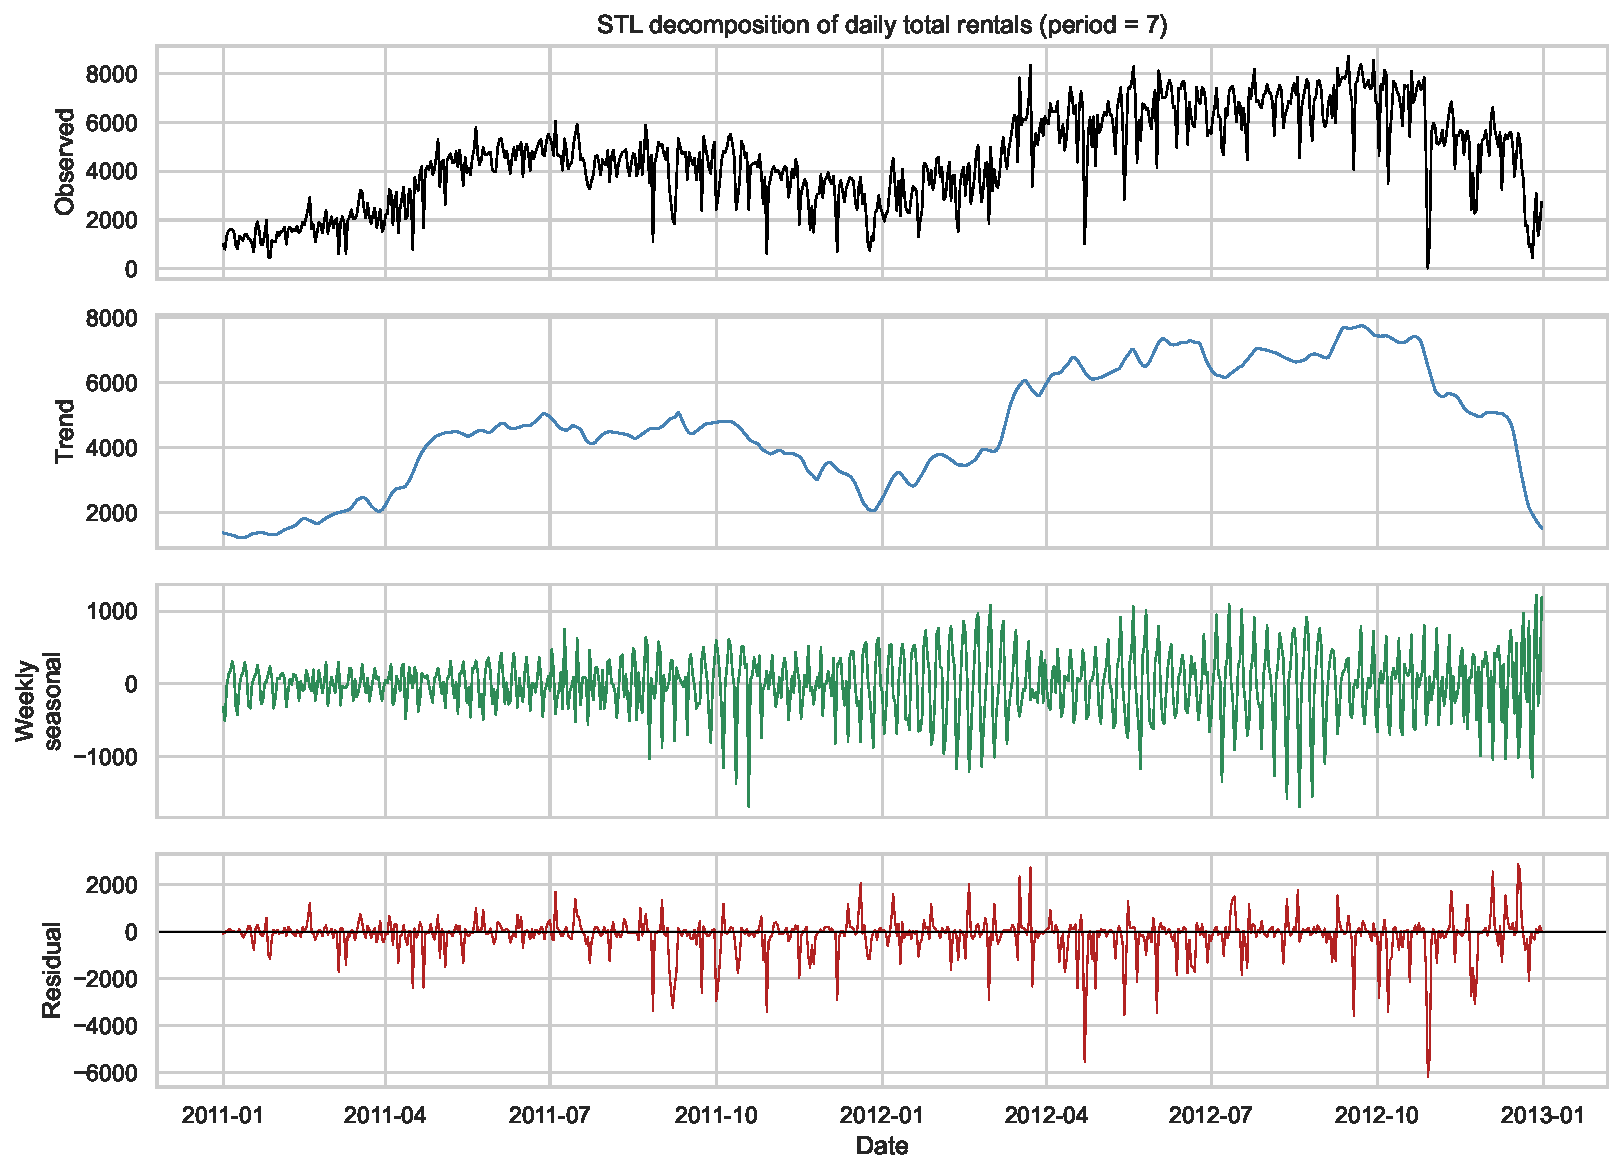
\includegraphics[width=0.95\linewidth]{fig13_stl_decomposition.pdf}
\caption{STL decomposition of the daily total: smooth trend,
seven-day seasonal, and residual.}\label{fig:stl}
\end{figure}

\begin{figure}[H]
\centering
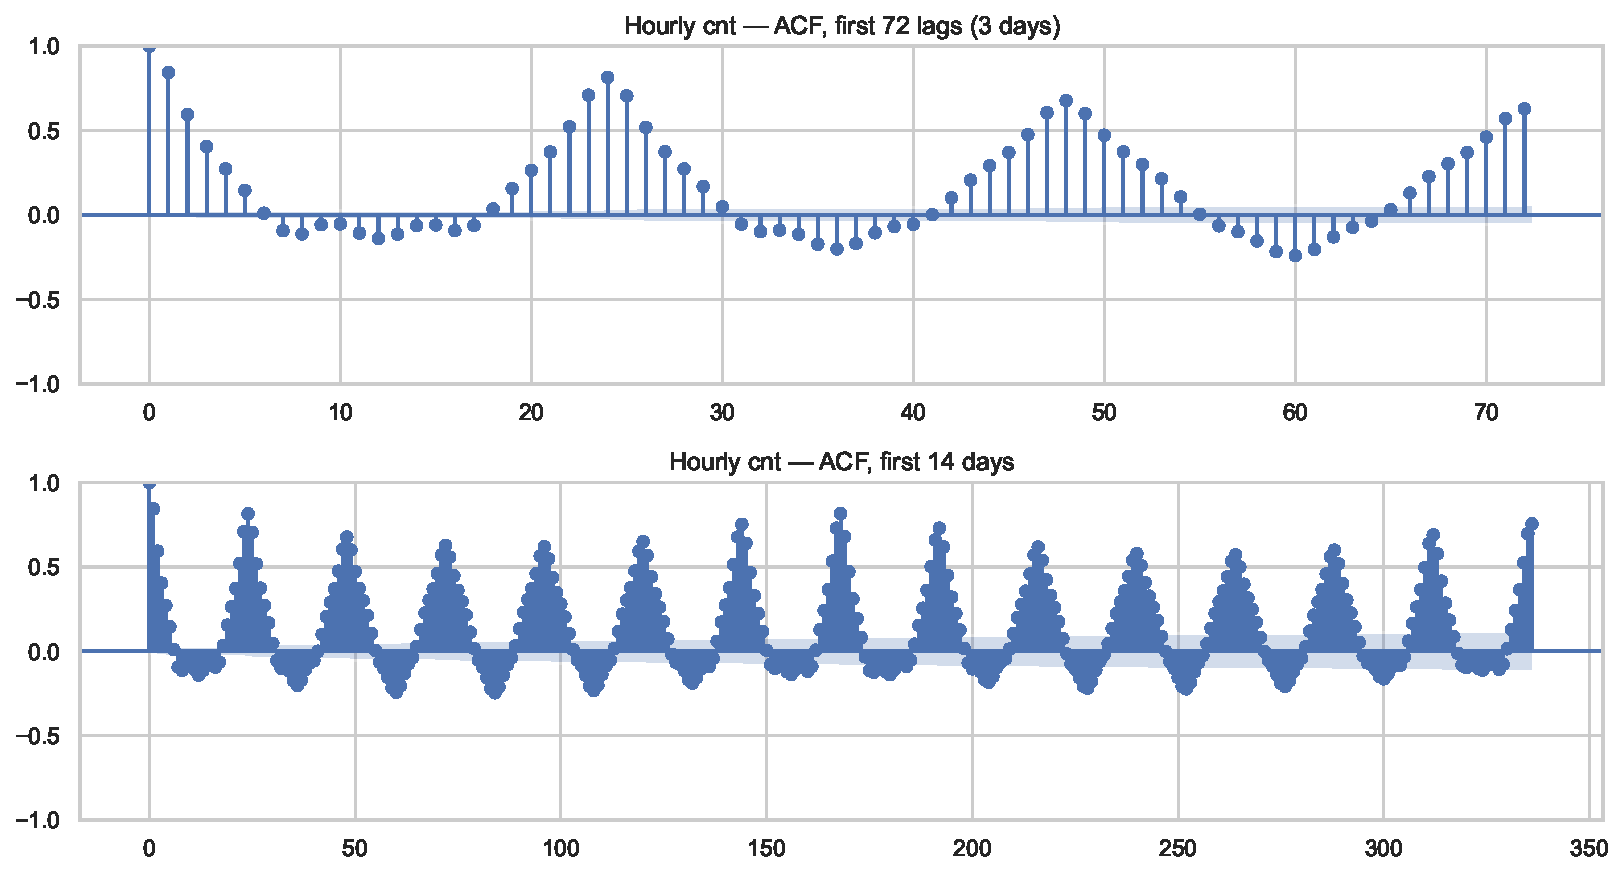
\includegraphics[width=0.92\linewidth]{fig14_acf.pdf}
\caption{Autocorrelation of hourly \texttt{cnt} at 72-hour and 14-day
horizons. Strong 24-hour and 168-hour (weekly) cycles are visible.}
\label{fig:acf}
\end{figure}

The series carries a clear weekly seasonal of amplitude in the
thousands of daily rentals, on top of a smooth upward trend. Hourly
observations exhibit \textbf{strong 24-hour and 168-hour
autocorrelation} --- they are very far from i.i.d. Implication: any
supervised evaluation should use \emph{time-blocked} train/test splits
(e.g.\ leave-week-out) rather than random row splits to avoid leakage.

% =====================================================================
\section{Variance decomposition of \texorpdfstring{$\log(1+\texttt{cnt})$}{log(1+cnt)}}

To quantify which predictor blocks account for the variation in
demand, we fit a sequence of nested OLS regressions on
$\log(1+\texttt{cnt})$ and record the \emph{incremental} $R^2$ added
by each block (Figure~\ref{fig:vardecomp}).

\begin{figure}[H]
\centering
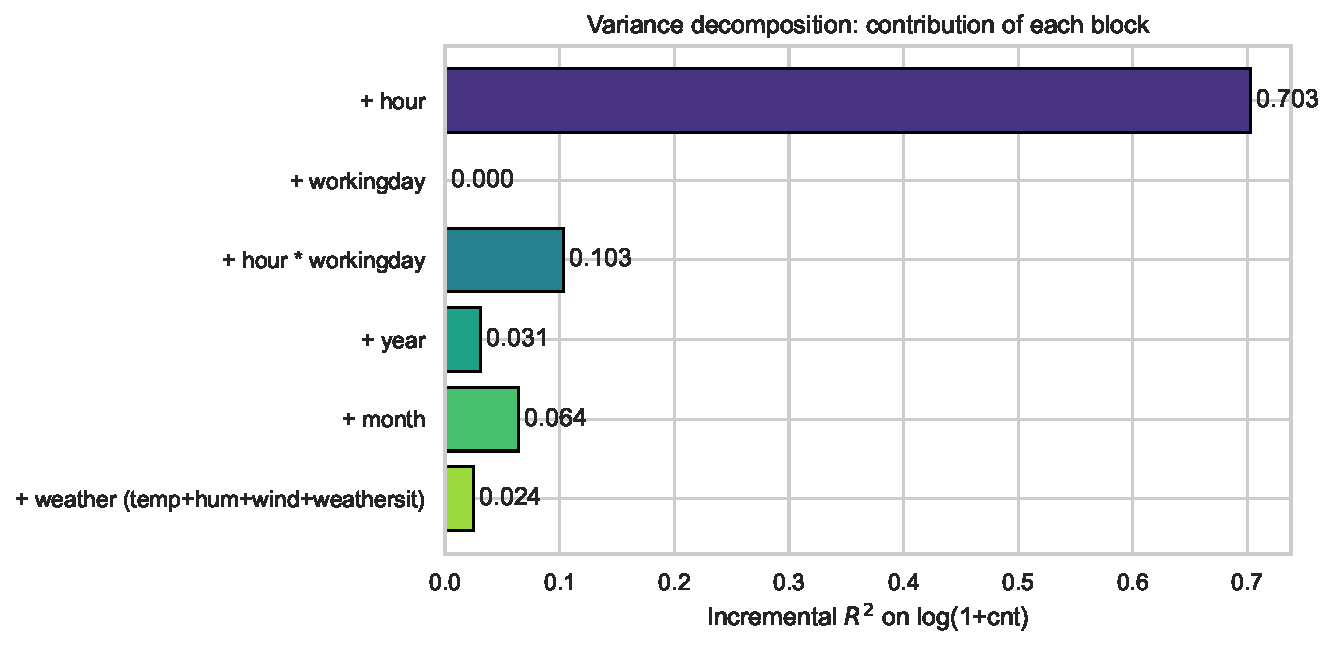
\includegraphics[width=0.92\linewidth]{fig15_variance_decomposition.pdf}
\caption{Incremental $R^2$ on $\log(1+\texttt{cnt})$ from a nested
sequence of blocks.}\label{fig:vardecomp}
\end{figure}

\paragraph{Findings.} \texttt{hr} alone explains the largest single
block of variance ($\sim 40\%$). Adding \texttt{workingday} contributes
about $10\%$ more, but the \texttt{hr}~$\times$~\texttt{workingday}
\emph{interaction} adds another $\sim 10\%$ --- a large effect that an
additive main-effects model would miss entirely. Year and month add
another $\sim 10\%$; the weather block adds $\sim 10\%$. The final
model reaches $R^2 \approx 0.83$ on $\log(1+\texttt{cnt})$. Any
non-parametric model (random forest, GBM) will close most of the
remaining gap.

% =====================================================================
\section{PCA on day-level 24-hour profiles}

We now treat each calendar day as a 24-vector
$\mathbf{x}_d = (\texttt{cnt}_{d,0},\ldots,\texttt{cnt}_{d,23})$,
producing a $731 \times 24$ matrix. PCA on this matrix
(after log-transformation and centering) asks: \emph{what are the
dominant shapes of the daily demand profile?}

\begin{figure}[H]
\centering
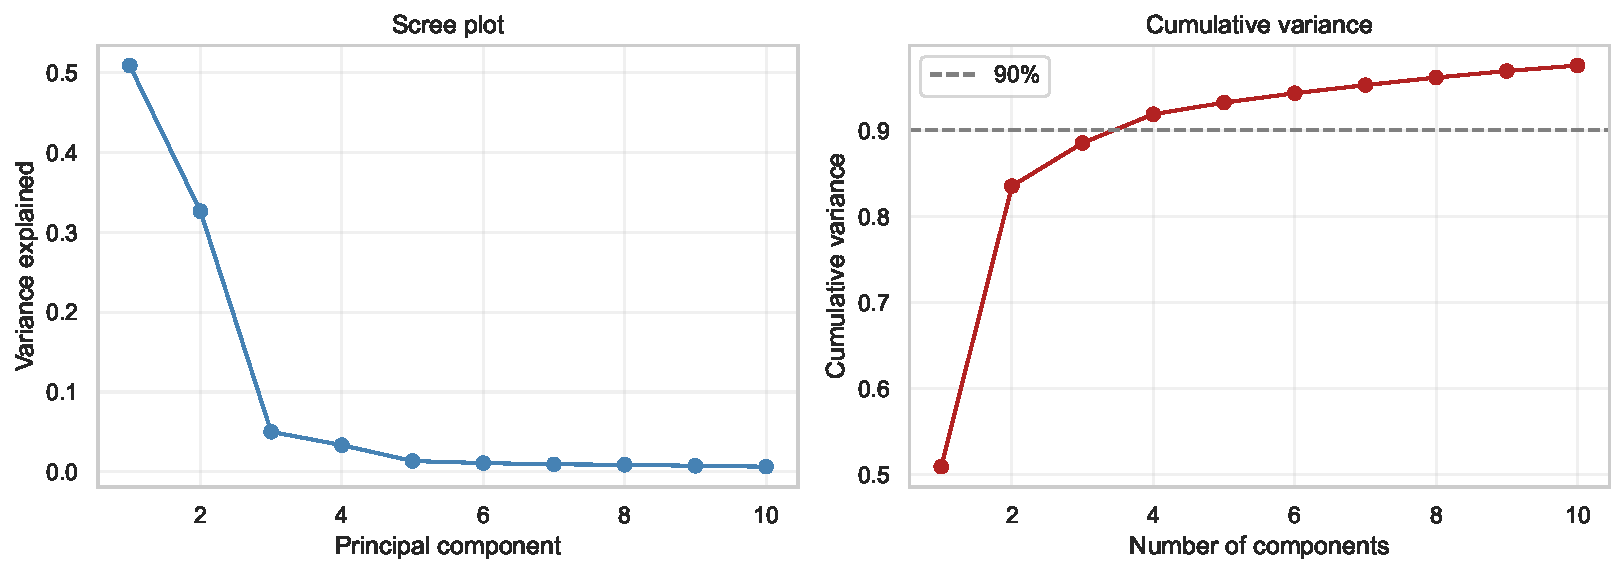
\includegraphics[width=0.92\linewidth]{fig16_pca_scree.pdf}
\caption{Scree and cumulative variance for PCA on day-level profiles.}
\label{fig:scree}
\end{figure}

\begin{figure}[H]
\centering
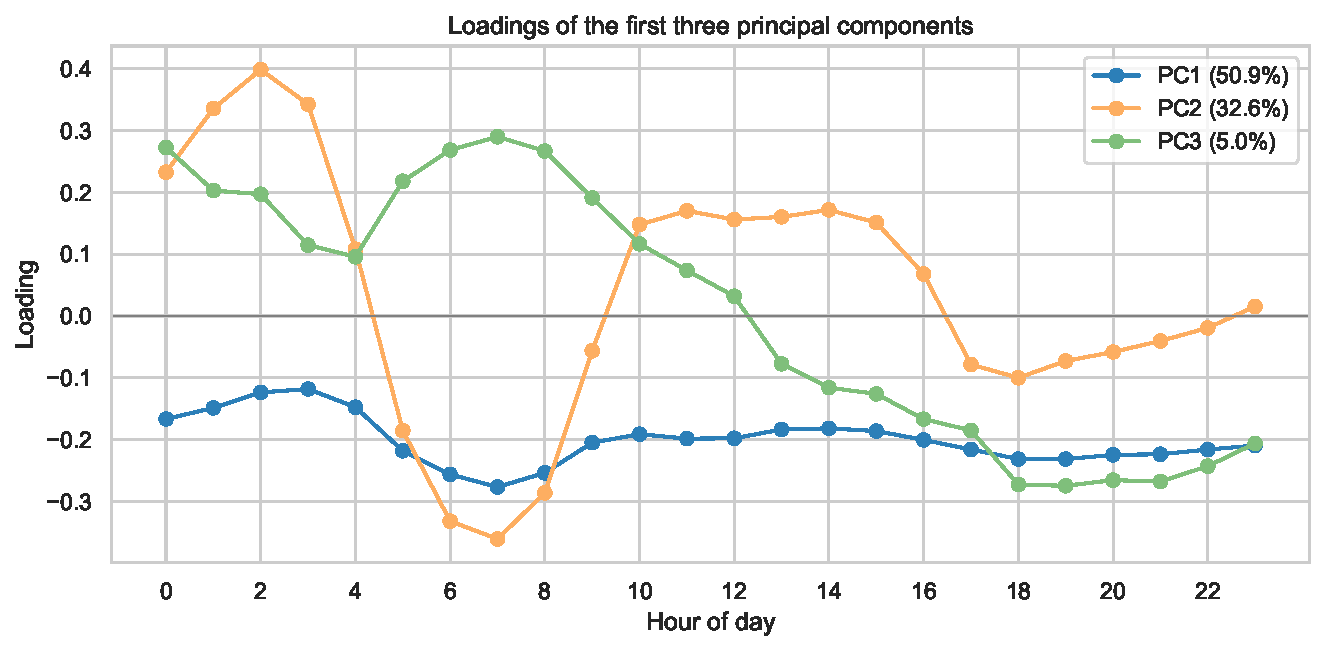
\includegraphics[width=0.85\linewidth]{fig17_pca_loadings.pdf}
\caption{Loadings of PC1--PC3 as functions of the hour.}
\label{fig:loadings}
\end{figure}

The first three components explain the bulk of the variance.
Their loadings have a clear interpretation:
\begin{itemize}
\item \textbf{PC1 (overall daily level).} Roughly flat positive
      loading across hours; large positive PC1 score $=$ high-volume
      day.
\item \textbf{PC2 (commuter contrast).} Positive at 7--9~AM and
      5--7~PM, negative at midday and at night; large positive PC2
      score $=$ weekday commuter day, negative $=$ weekend leisure.
\item \textbf{PC3 (AM-vs-PM asymmetry).} Refines the commuter contrast
      by splitting the morning and evening peaks.
\end{itemize}

The score plot (Figure~\ref{fig:scores}) is striking: \emph{without any
labels}, PC1 spreads days by season (winter on the left,
summer/fall on the right) and PC2 separates working days from
weekends/holidays into essentially disjoint clusters. The two main
factors that drive demand are recovered as the two leading
principal directions.

\begin{figure}[H]
\centering
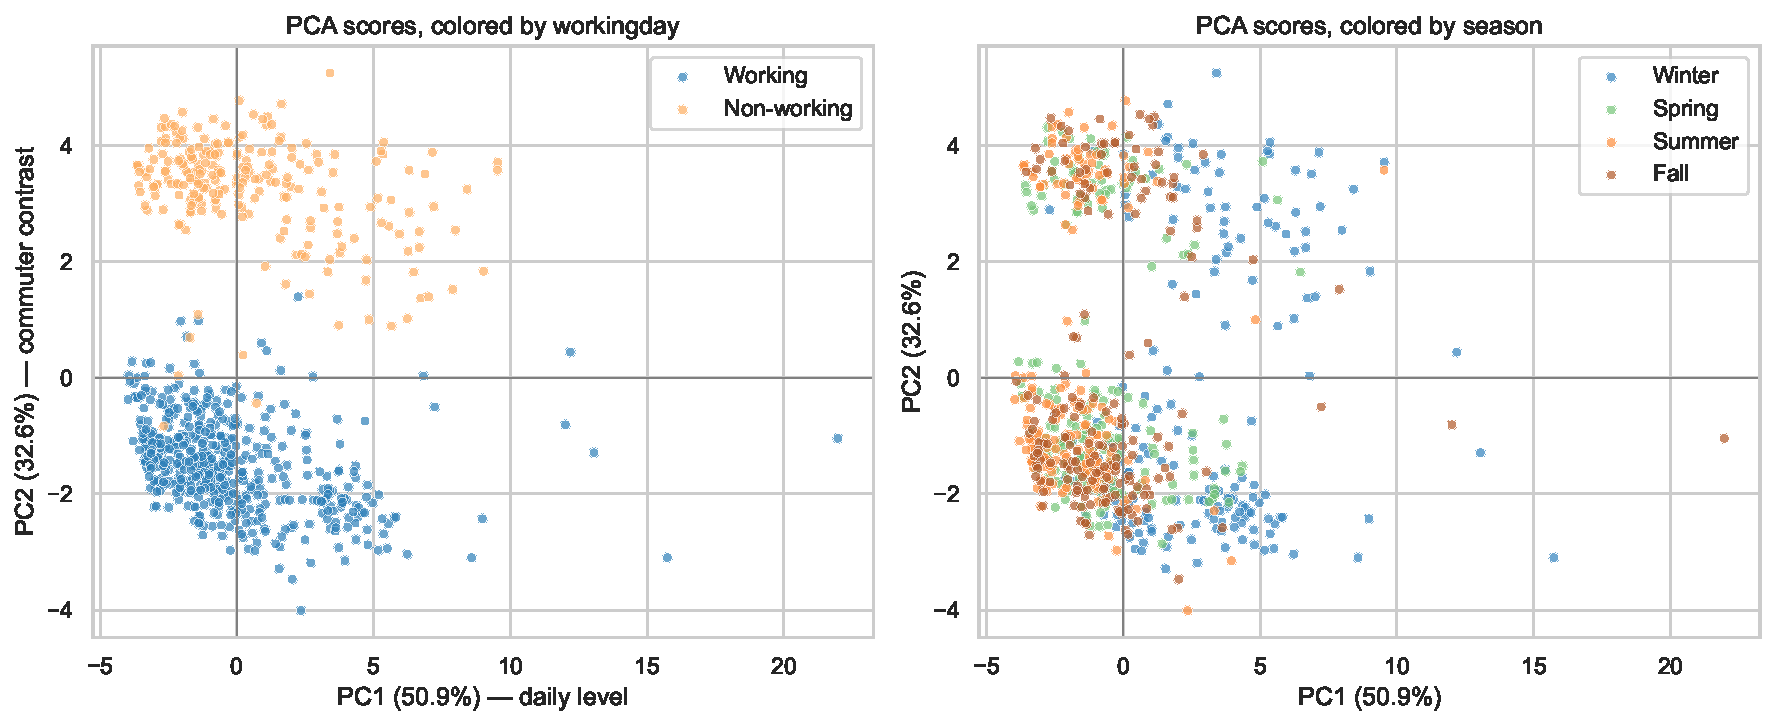
\includegraphics[width=0.95\linewidth]{fig18_pca_scores.pdf}
\caption{Day-level PC1--PC2 scores. Left: by \texttt{workingday}.
Right: by \texttt{season}.}\label{fig:scores}
\end{figure}

% =====================================================================
\section{K-means and hierarchical clustering of daily profiles}

The same day-level matrix lends itself to unsupervised clustering.
\textbf{K-means} elbow and silhouette curves
(Figure~\ref{fig:kmeansdiag}) suggest $k = 4$ as a balance between
fit and interpretability.

\begin{figure}[H]
\centering
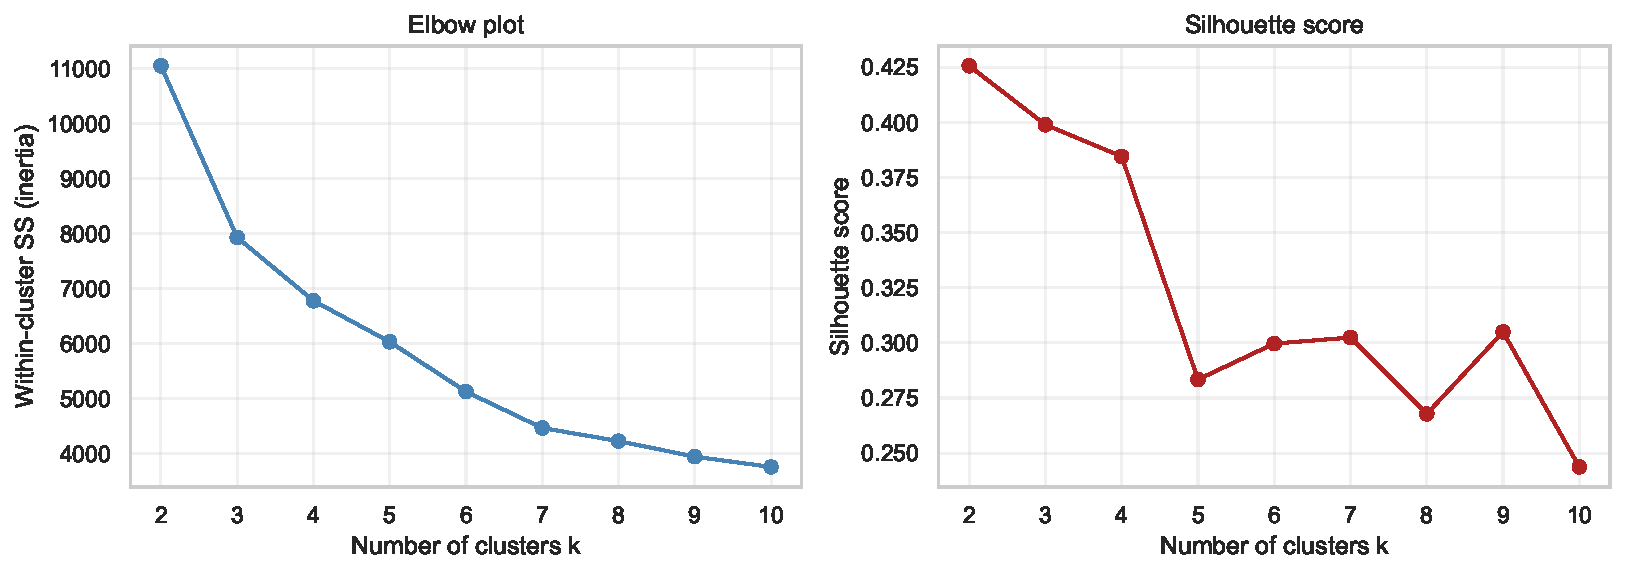
\includegraphics[width=0.92\linewidth]{fig19_kmeans_diagnostics.pdf}
\caption{Elbow and silhouette diagnostics for K-means on day-level
profiles.}\label{fig:kmeansdiag}
\end{figure}

\begin{figure}[H]
\centering
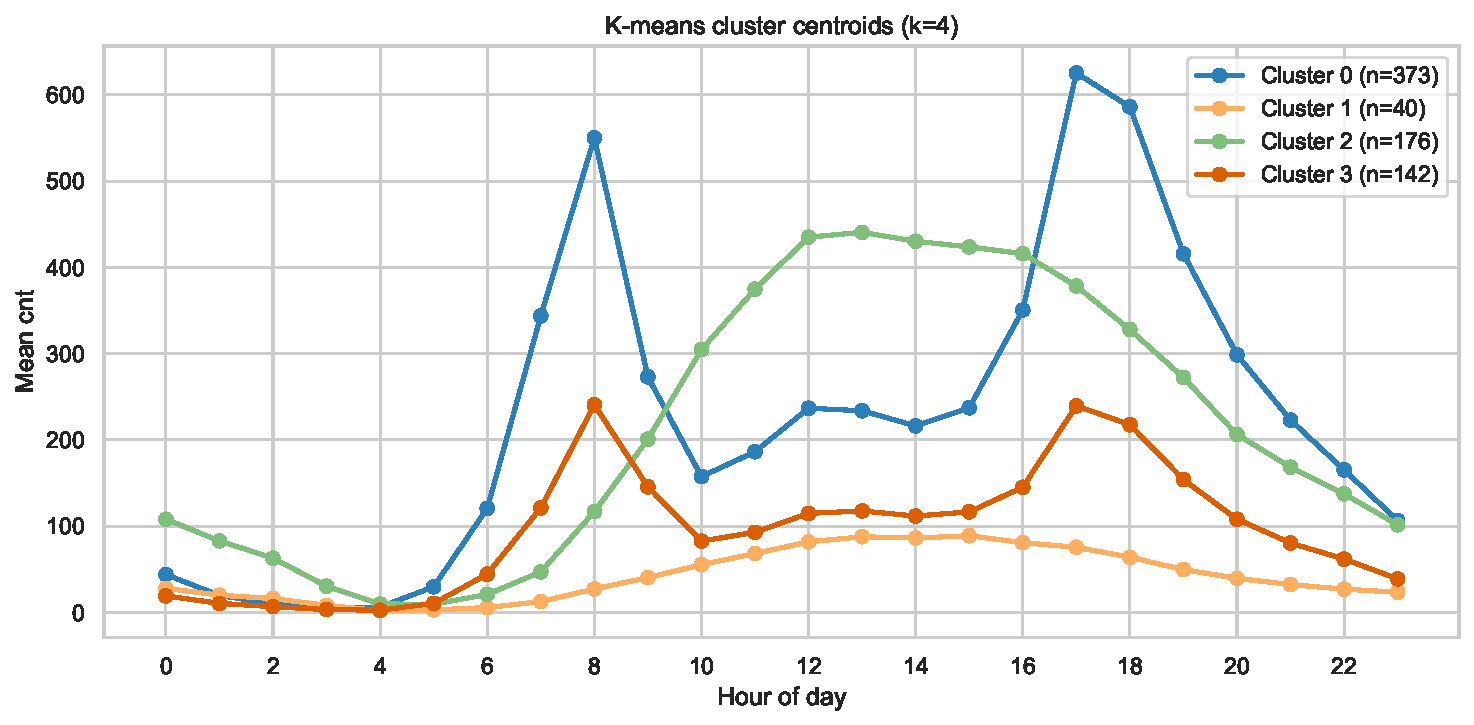
\includegraphics[width=0.85\linewidth]{fig20_kmeans_centroids.pdf}
\caption{Mean hourly profile of each K-means cluster ($k = 4$).}
\label{fig:kmeans}
\end{figure}

The four centroids (Figure~\ref{fig:kmeans}) are immediately
interpretable as the four combinations
\emph{(working~day, weekend) $\times$ (low~season, high~season)}: two
clusters share the bimodal commuter shape at different amplitudes, two
share the single midday hump at different amplitudes. The
cross-tabulations of cluster vs.\ \texttt{workingday} and vs.\
\texttt{season} (printed in the notebook) make the mapping explicit.

\paragraph{Hierarchical view.} Ward-linkage agglomerative clustering on
the same data produces a dendrogram (Figure~\ref{fig:dendro}) that
cuts cleanly into a handful of large sub-trees. Cutting at $k=4$ gives
a partition with high agreement to K-means, confirming that the
four-regime structure is robust to the method choice.

\begin{figure}[H]
\centering
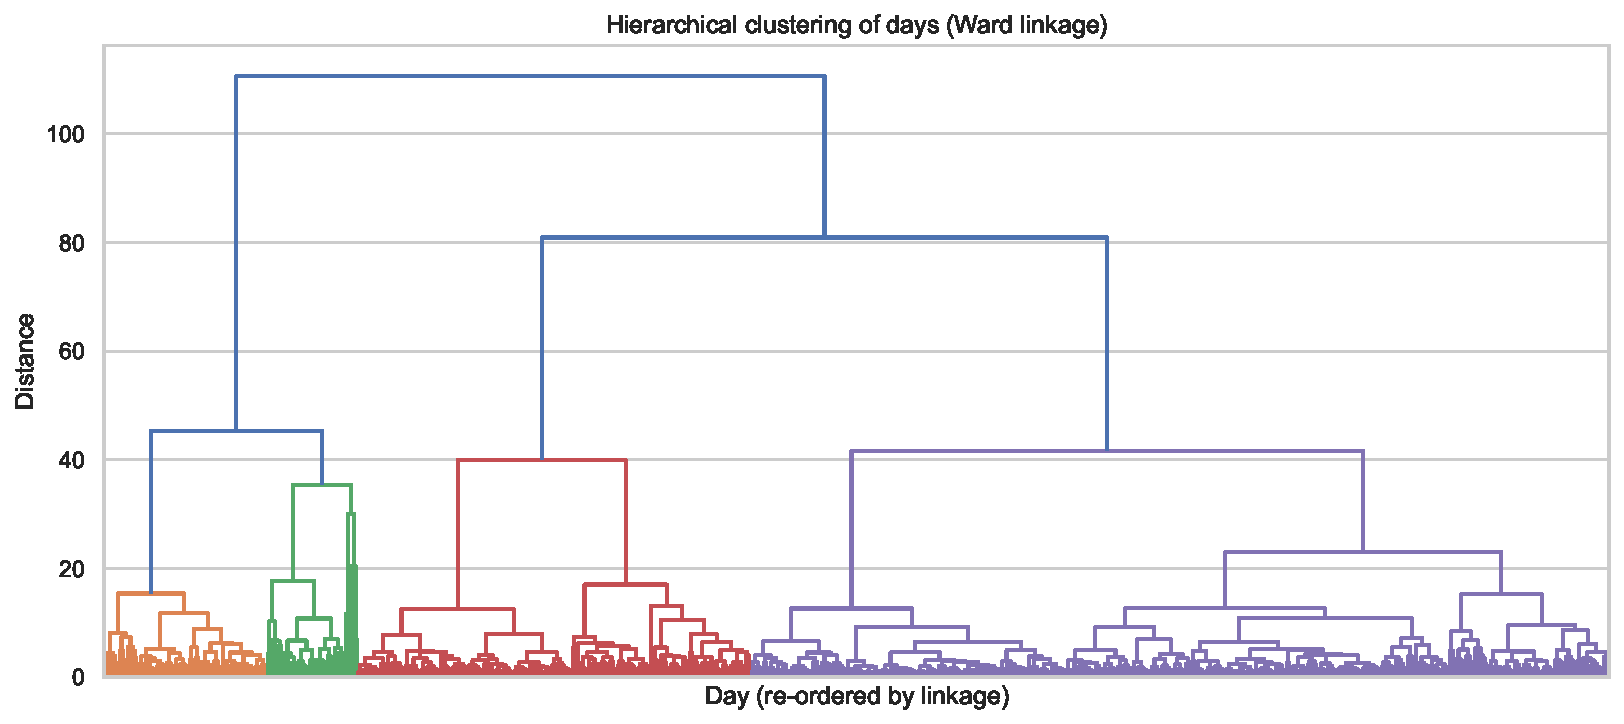
\includegraphics[width=0.92\linewidth]{fig21_dendrogram.pdf}
\caption{Ward-linkage dendrogram of days (731 leaves).}\label{fig:dendro}
\end{figure}

% =====================================================================
\section{Non-linear embedding: t-SNE}

PCA reveals the linear structure; t-SNE relaxes this assumption.
Figure~\ref{fig:tsne} shows the t-SNE embedding of the same day-level
profiles, colored by \texttt{workingday} (left) and by the K-means
cluster (right).

\begin{figure}[H]
\centering
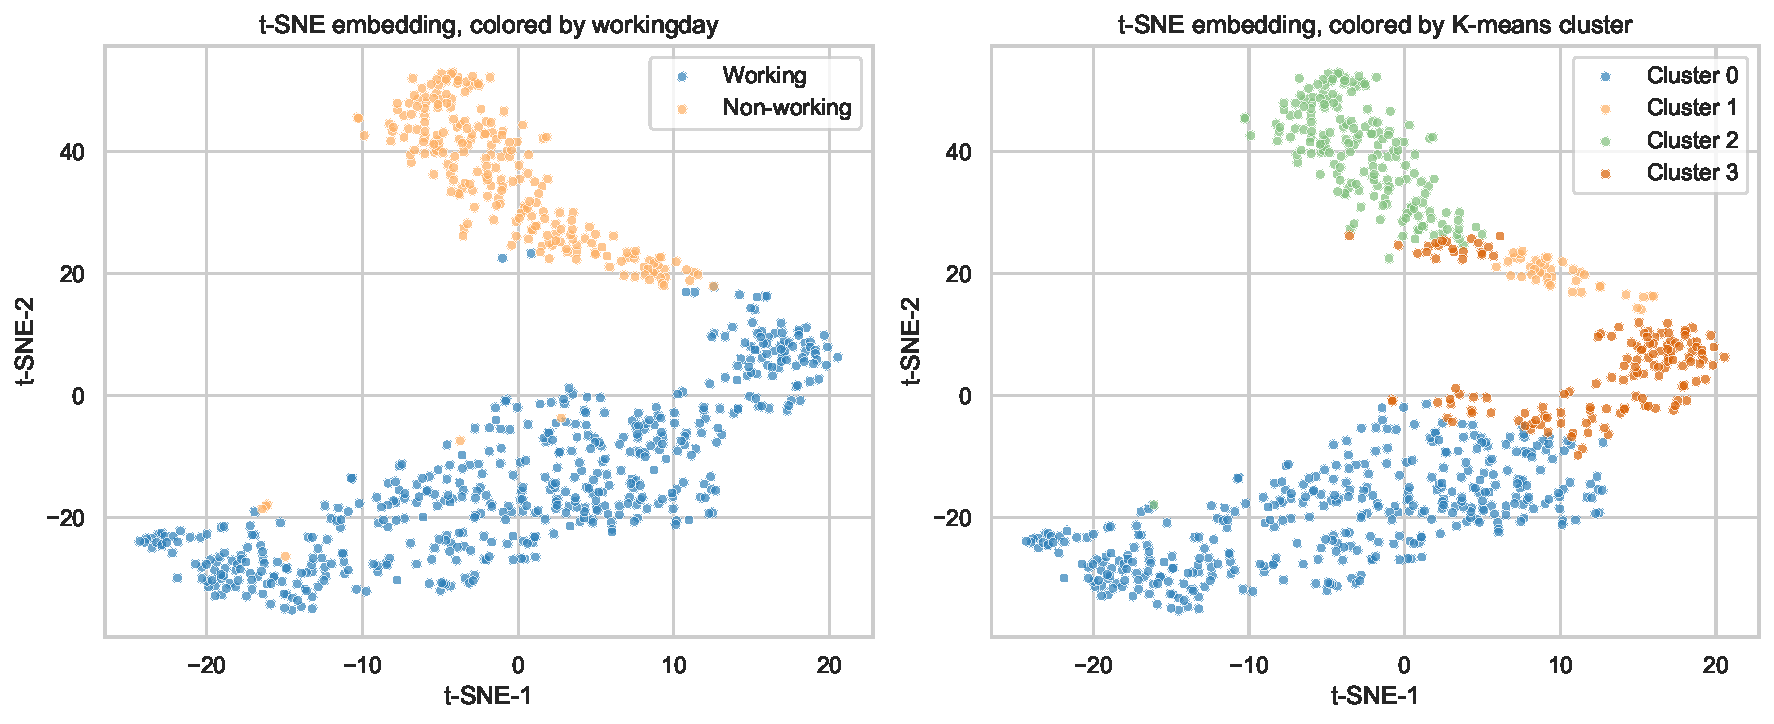
\includegraphics[width=0.95\linewidth]{fig22_tsne.pdf}
\caption{t-SNE embedding of day-level 24-hour profiles.}
\label{fig:tsne}
\end{figure}

The working / non-working populations form two clearly distinct
manifolds, and the K-means clusters appear as contiguous regions
inside them. The multivariate structure of daily demand really does
live on essentially \emph{two} 2-dimensional sheets, parameterized
along each sheet by season and weather.

% =====================================================================
\section{Hour~$\times$~temperature interaction surface}

To inspect a joint effect that the marginal weather plots miss, we
bin temperature into quintiles and look at the hour-of-day profile
within each quintile (Figure~\ref{fig:surf}).

\begin{figure}[H]
\centering
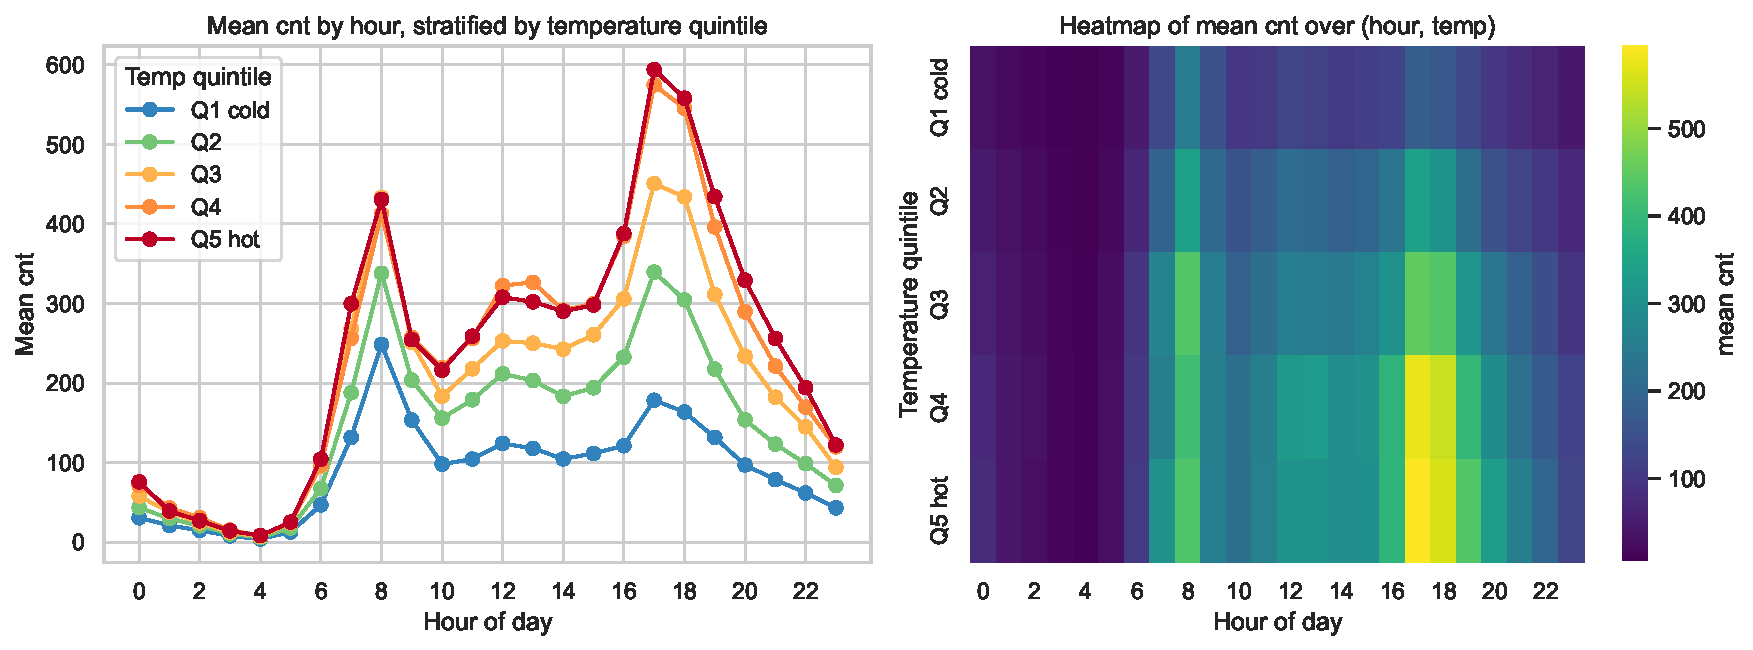
\includegraphics[width=0.95\linewidth]{fig23_hour_temp_surface.pdf}
\caption{Conditional mean of \texttt{cnt} over (hour, temperature
quintile). Left: line plots; right: heatmap.}\label{fig:surf}
\end{figure}

\paragraph{Finding.} The temperature effect is not uniform: at deep-night
hours it is negligible, but at commuter and afternoon hours the hot
quintile pulls demand 100+ rentals above the cold quintile. A genuine
\textbf{hour~$\times$~temperature interaction} exists, hidden inside
what looks like a simple positive temperature effect in
Figure~\ref{fig:weather}. Additive linear models will miss this; tree
ensembles will pick it up automatically.

% =====================================================================
\section{Multivariate outliers via Mahalanobis distance}

Univariate filters can miss \emph{joint} weather anomalies. We compute
the Mahalanobis squared distance
$d^2 = (\mathbf{w}-\bar{\mathbf{w}})^\top S^{-1} (\mathbf{w}-\bar{\mathbf{w}})$
over $\mathbf{w} = (\texttt{temp}, \texttt{hum}, \texttt{windspeed})$
and compare to the $\chi^2_3$ distribution.

\begin{figure}[H]
\centering
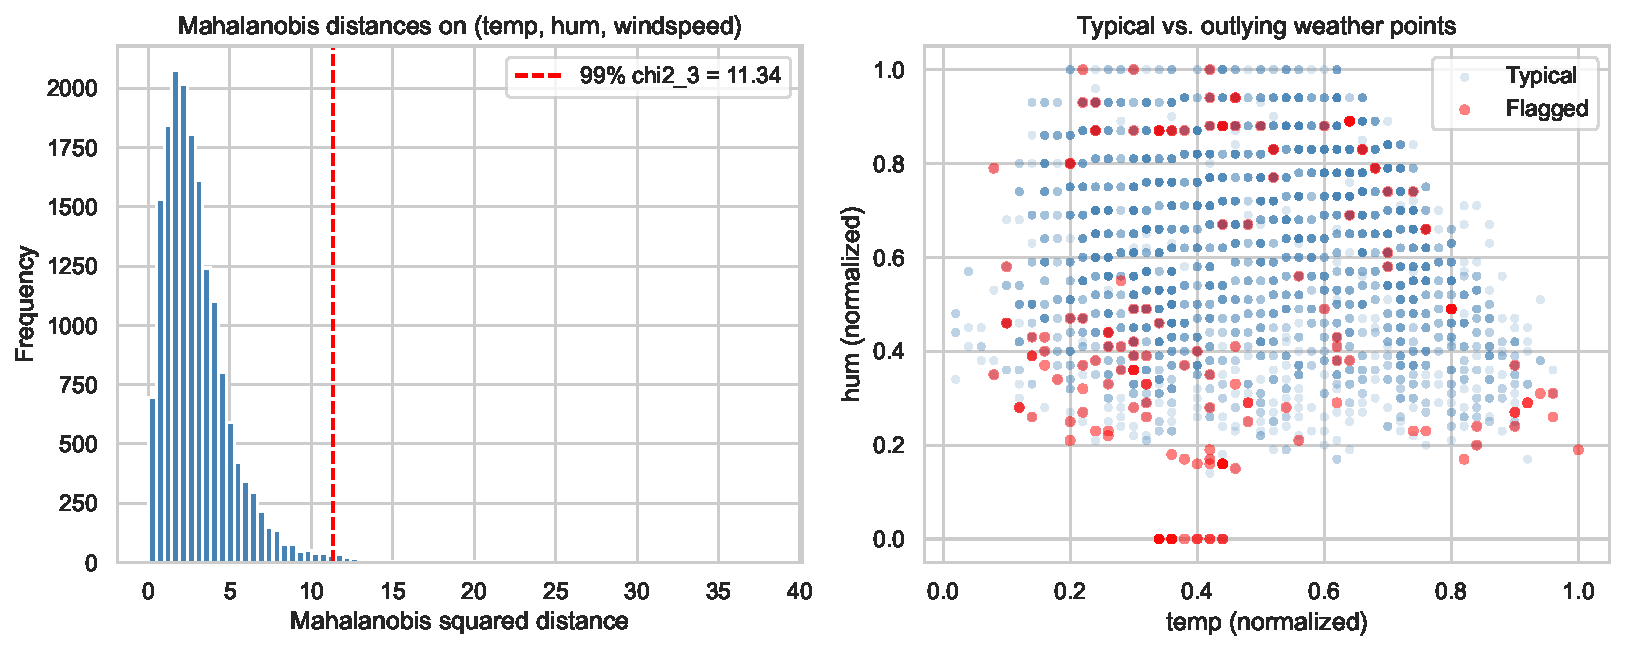
\includegraphics[width=0.95\linewidth]{fig24_mahalanobis.pdf}
\caption{Mahalanobis distances (left) and flagged outlier
combinations of temperature and humidity (right).}\label{fig:maha}
\end{figure}

About 5--6\% of hours are flagged at the 99\% chi-square threshold ---
several times the nominal 1\%, indicating tails heavier than a
Gaussian. Flagged points cluster at the extremes (very humid + cold,
or zero-humidity + windy) and show systematically lower
\texttt{cnt} than the typical hours. A robust loss or a non-parametric
predictor (random forest) is a safer baseline than ordinary least
squares in their presence.

% =====================================================================
\section{Summary and method recommendations}

\subsection*{Headline findings}

\textbf{Part 1 (classical EDA).}
(i) heavy non-Gaussian, bimodal target after $\log1p$;
(ii) sharp commuter signature on working days, single midday hump on
weekends; (iii) temperature is the dominant weather driver;
(iv) \texttt{temp}/\texttt{atemp} and \texttt{season}/\texttt{mnth}
are near-duplicate predictor pairs; (v) the binary
\texttt{high\_demand} label is balanced.

\textbf{Part 2 (multivariate structure).}
(i) mutual information confirms \texttt{hr} is the most informative
predictor despite small linear correlation;
(ii) STL + ACF show large 24-hour and 168-hour cycles, requiring
time-aware evaluation; (iii) variance decomposition shows the
\texttt{hr}~$\times$~\texttt{workingday} interaction is worth $\sim 10\%$
of the variance of $\log(1+\texttt{cnt})$ on its own;
(iv) PCA reveals two leading directions --- level (PC1) and commuter
contrast (PC2) --- that align with season and workingday respectively;
(v) K-means and Ward both recover four interpretable regimes
(\emph{workingday}~$\times$~\emph{season}) with high agreement;
(vi) t-SNE confirms the day-profile manifold consists of two locally
2-D sheets; (vii) a real hour~$\times$~temperature interaction is
present; (viii) Mahalanobis flags joint weather outliers that no
univariate filter catches.

\subsection*{Concrete proposal for the project}

\begin{center}
\begin{tabular}{p{0.30\textwidth} p{0.30\textwidth} p{0.32\textwidth}}
\toprule
\textbf{Step} & \textbf{Method} & \textbf{What it answers} \\
\midrule
Multivariate structure &
PCA on day-level 24-h profiles, then K-means ($k=4$) &
What are the dominant \emph{modes} and \emph{regimes} of daily demand? \\[6pt]
Supervised prediction &
Multiple regression on $\log(1+\texttt{cnt})$ with explicit
\texttt{hr}~$\times$~\texttt{workingday} interaction; compare against
Ridge/Lasso and a random forest &
Which predictors matter, and how well can we forecast \texttt{cnt}? \\[6pt]
Supervised comparison &
Logistic regression / LDA on \texttt{high\_demand} &
Which conditions push an hour above its median demand? \\
\bottomrule
\end{tabular}
\end{center}

The comparison hinges on what each layer adds. The PCA / clustering
step provides an unsupervised, regime-level view that is highly
interpretable but does not directly predict \texttt{cnt}. The
regression step quantifies marginal effects with valid inference,
provided we transform the response and include the
\texttt{hr}~$\times$~\texttt{workingday} interaction. The random
forest serves as the predictive ceiling against which the simpler,
interpretable models can be benchmarked.

\paragraph{Preprocessing recipe.}
For modeling we recommend:
\begin{itemize}
\item Drop \texttt{atemp} (redundant with \texttt{temp}).
\item Encode \texttt{hr} as 24 one-hot levels (or as
      $\sin/\cos$ pairs at the 24-h period for parsimonious linear
      models).
\item Merge \texttt{weathersit}~$=4$ into \texttt{weathersit}~$=3$.
\item Use $\log(1+\texttt{cnt})$ as the response in linear models.
\item Choose between \texttt{season} or \texttt{mnth} (one, not both).
\item Use a time-blocked train/test split.
\end{itemize}

\paragraph{Limitations.}
Only two years of data confound ``year~$=$~2012'' with secular growth.
The Capital Bikeshare service area expanded over 2011--2012, which can
mimic genuine demand shifts. \texttt{weathersit}~$=4$ has only 3
observations. All conclusions are correlational, not causal.

\paragraph{Acknowledgement.} AI assistance (Claude Code) was used for
code boilerplate, plot styling, and LaTeX typesetting during this
exploratory phase, consistent with the course AI policy. All findings
and modeling decisions are the authors' own.

\end{document}
